%Title of section
\section{容器负载预测模型}

\subsection{模型结构}

\begin{frame}
\frametitle{模型结构}
\framesubtitle{引言}
\begin{itemize}
    \item 单值预测模型:ARIMA、Kalman滤波、神经网络、……
    \begin{itemize}
        \item \textbf{误差敏感} $\Rightarrow$ \textbf{决策失效}
        \item \textbf{鲁棒性差} $\Rightarrow$ \textbf{决策过度}
    \end{itemize}
    \item 区间预测模型:贝叶斯、回归模型、随机森林、……
    \begin{itemize}
        \item \textbf{预测区间} $\Rightarrow$ \textbf{目标不确定性(包含误差)}
        \item \textbf{区间置信度} $\Rightarrow$ \textbf{适合决策}
        \item \alert{\textbf{先预测再扩展为区间} $\Rightarrow$ \textbf{先验假设}}
        \item \alert{\textbf{相同分布假设} $\nRightarrow$ \textbf{适应不同类型负载}}
    \end{itemize}
    \item 基于趋势感知的区间预测模型:SAC-GPSO-SVM
    \begin{itemize}
        \item \textbf{趋势感知} $\Rightarrow$ \textbf{平稳型、趋势型和周期型负载}
        \item \textbf{区间构造} $\Rightarrow$ \textbf{针对不同负载类型}
        \item \textbf{区间预测} $\Rightarrow$ \textbf{先构建区间再预测}(\sout{先预测再扩展为区间})
        \item \textbf{实时预测} $\Rightarrow$ \textbf{预测效率(模型训练和超参数优化)}
    \end{itemize}
\end{itemize}
\end{frame}

\begin{frame}
\frametitle{模型结构}
\framesubtitle{示意图}
\begin{columns}
\begin{column}{0.4\textwidth}
\begin{figure}[htb]
\centering

\includegraphics[scale=0.3]{figures/fig6_sac-gpso-svm.jpg}
\caption{基于趋势感知的区间预测模型}
\label{fig:fig6}
\end{figure}
\end{column}
\begin{column}{0.6\textwidth}
\begin{figure}[htb]
\centering
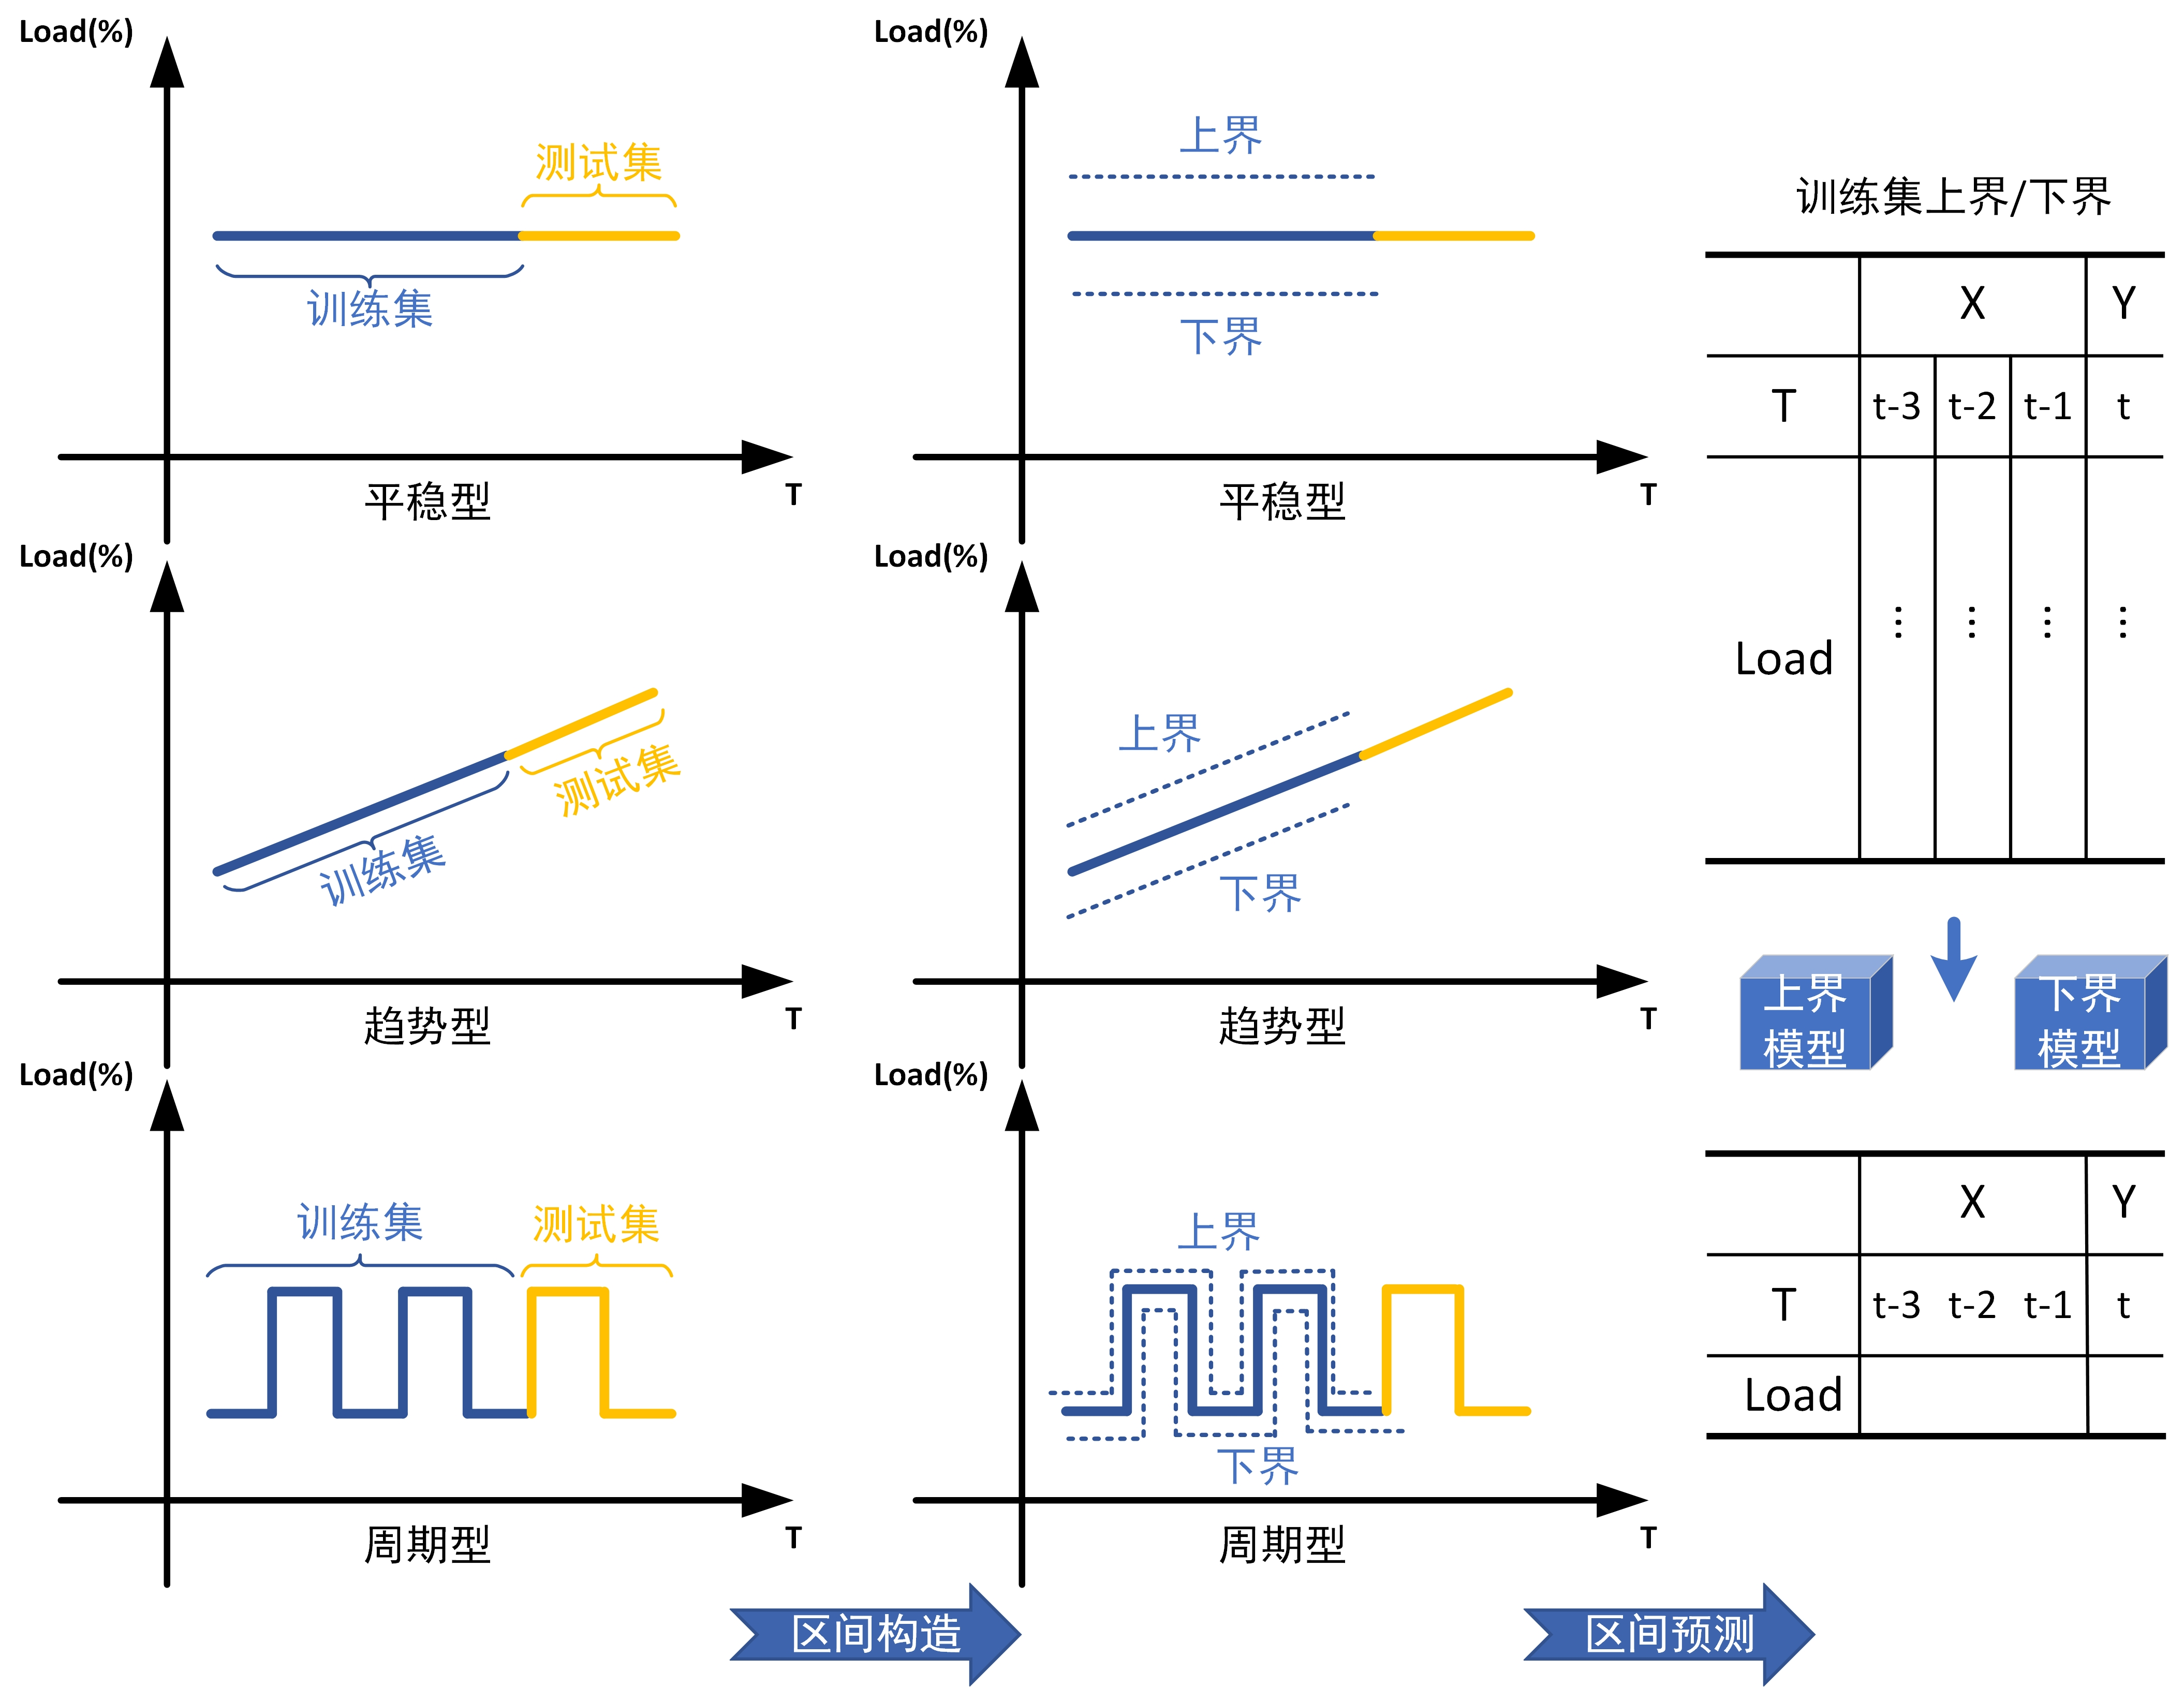
\includegraphics[scale=0.38]{figures/fig7_predict_process.jpg}
\caption{模型预测过程}
\label{fig:fig6}
\end{figure}
\end{column}
\end{columns}
\end{frame}

\subsection{趋势感知}

\begin{frame}
\frametitle{趋势感知}
\framesubtitle{定义}
\end{frame}

\begin{frame}
\frametitle{趋势感知}
\framesubtitle{频谱特征分析}
\end{frame}

\begin{frame}
\frametitle{趋势感知}
\framesubtitle{自相关系数分析}
\end{frame}

\subsection{区间构造}

\begin{frame}
\frametitle{区间构造}
\end{frame}


\subsection{区间预测}

\begin{frame}
\frametitle{区间预测}
\end{frame}


\subsection{实验结果与分析}

\begin{frame}
\frametitle{实验结果与分析}
\end{frame}